\documentclass[10pt]{article}
\usepackage[utf8]{inputenc}
\usepackage[a4paper, left=25mm, top=25mm, right=25mm, bottom=25mm]{geometry}
\usepackage[utf8]{inputenc}
\usepackage{listings}
\usepackage[english]{babel,isodate}
\usepackage[pdftex, pdfauthor={Steven Tang, Qifan Deng}, pdftitle={COMP90024 - Cloud and Cluster Computing 2020, Assignment 1}, pdfsubject={COMP90024 Assignment},hidelinks]{hyperref}
\usepackage{listings}
\usepackage{pgfplots} 
\usepackage[justification=centering]{caption}
\usepackage{enumitem}
\usepackage{float}

\setlength{\columnsep}{20pt}
\setlength{\parindent}{8pt}
\setlength{\parskip}{3pt}

\pgfplotsset{compat=1.16}

\title{COMP90024 - Cloud and Cluster Computing, Assignment 1\\HPC Twitter Processing }
\author{
  Steven Tang (832031)\\
  \texttt{stevent2@student.unimelb.edu.au}\and
  Qifan Deng (1077479)\\
  \texttt{qifand@student.unimelb.edu.au} }
\date{\printdayoff\normalsize\today}

\begin{document}
\sloppy
\twocolumn
\maketitle

\section{Introduction}
Project 1 is about developing a parallel application to process a large Twitter dataset. A hybrid approach using MPI with OpenMP was taken. 

The structure of this report is as follows. \hyperref[design]{Section 2} outlines the architecture of the developed application, with rationale given for critical aspects of the design. \hyperref[results]{Section 3} presents the performance of the application, with results discussed and analysed. Finally, potential improvements are suggested in \hyperref[improvements]{section 4}. 

\subsection{Compilation \& invocation}
\subsubsection{Dependencies}
\begin{itemize}
  \setlength\itemsep{1pt}
    \item make, g++
    \item MPI
    \item OpenMP
    \item rapidjson (source included)
\end{itemize}

\subsubsection{Compilation and invocation}
\begin{verbatim}
$ make
$ mpirun [-np <n>] --bind-to none \
    ./tp <inputTwitter.json> <lang.csv>
\end{verbatim}

\section{Design and architecture}
\label{design}
\subsection{Assumptions made}
Below, some assumptions and their implications are listed:

\begin{itemize}[topsep=2pt]
    \setlength\itemsep{1pt}
   
    \item The assignment's focus is not on the performance of the application.
    Only trivial performance optimisations were performed. 
   
    \item It is not essential to optimise for the scenario where only one thread is available for a particular process. Currently, a sequential merging step is performed to combine results from multiple threads. This step can be skipped if there is only one thread. 

    \item The data is assumed to be in the format that is defined in \texttt{bigTwitter.json}.
    That is, excluding the first and last lines, each line (delimited by \texttt{CRLF}) is a tweet in JSON\footnote{\url{https://developer.twitter.com/en/docs/tweets/data-dictionary/overview/tweet-object}},
    with a possible trailing comma. \\
    Additionally, such files may be truncated at the end of particular lines, as is the case with \texttt{(tiny|small)Twitter.json}. 
    
    \item Input files can be concurrently read by multiple processes and threads.
\end{itemize}

% - data structure
% - purpose of assignment is not focused on making processing code run faster
% - did not dive into performance of json parsing
% - do not optimise for one core, one thread (multiple redundant merging steps)

\subsection{Overview}
The implemented application can be logically separated into three primary components. 

At the top level, the input Twitter file is subdivided into $n$ evenly-sized chunks, one for each MPI process. 
To achieve thread parallelism, these chunks are then further subdivided, 
with individual lines (or tweets in JSON) in those subdivisions parsed and processed. % in threads
Results (stored in hashmaps) are then combined at both the thread and process levels to form the final result. 
% Hashmaps are used to count frequencies. 

Because lines in the tweet file are not of fixed length and it would be expensive to determine and seek to the starting positions of particular lines, it was determined that it would be infeasible to perform divisions by using line numbers. Instead, divisions are performed at the byte level, with logic implemented to avoid duplicate processing of the same line. 

% - division of work (byte-level)
% - new line

\subsubsection{Process}
The division of the input file across multiple MPI processes is performed in \texttt{main.cpp}.
The code for combining and printing results is located in \texttt{combine.cpp}. 

To summarise, the following steps are taken:

\begin{enumerate}[topsep=2pt]
    %\setlength\itemsep{1pt}

    \item Read the language file (which stores mappings between language codes and names).
    \item Obtain the length of the input Twitter file.
    \item Divide the input file into even chunks. During this step, the start and end byte positions for each process is calculated, based on the length of the file, the number of MPI processes and the rank of the current process.
    \item Pass start and end positions to \texttt{threading.cpp} (see \ref{thread}), and obtain two result hashmaps as the return value.
    \item Processes with $\texttt{rank} > 0$ send their results to the master process (rank 0); the master process merges received results. 
    \item Format and print overall results.
\end{enumerate}

\subsubsection{Thread}\label{thread}
% The primary motivation behind using a threaded approach is to reduce the amount of communication that is required to combine the final results. 
The primary motivation behind using a threaded approach is to reduce the communication overhead that is incurred when there are many MPI processes (i.e. one for each core). 

In \texttt{threading.cpp}, the section of the input file that is allocated to the current process (indicated by start and end byte positions) is further subdivided. 
To reduce load imbalance at the thread level, sections are subdivided into 200MB chunks, as opposed to having further even divisions between threads. 

OpenMP is then used to schedule the parallel processing of the aforementioned chunks. 
During this process, lines in each chunk are extracted and passed to \texttt{line.cpp}, 
which extracts and merges results to the hashmap of the current thread. 
Once all the chunks have been processed, hashmaps from threads are merged in a critical section to form the overall result for the current process.

\subsubsection{Line}
Languages and hashtags are extracted and counted in \texttt{line.cpp}. 
Lines containing tweets are parsed into document objects (\texttt{DOM}) using  \texttt{RapidJson}\footnote{\url{https://rapidjson.org/}}, 
a fast and self-contained JSON parser. 

The language code is directly read from \texttt{DOM["doc"]["lang"]}, while for counting hashtags, the regular expression \texttt{"\#[$\backslash$d$\backslash$w]+"} is used. With this expression, only strings which start with a \texttt{"\#"} and consisting of alphanumeric characters and underscores are matched. Following this, the string is converted to lowercase.
When examining the output of initial iterations, it was discovered that strings like \texttt{\#1} and \texttt{\#echobox} were matched by the expression. 
While such hashtags are valid, they were found in the description fields of users and URLs respectively. 

To avoid these occurrences, two fields from the document were chosen. The first is \texttt{DOM["doc"]["entities"]["hashtags"]}\footnote{\url{https://developer.twitter.com/en/docs/tweets/data-dictionary/overview/entities-object\#hashtags}}, an array of hashtag objects, in which the string in \texttt{["text"]} is a hashtag which is then validated. %for valid hashtags.
% Every hashtag string will be matched again to filter those not valid, e.g. foreign language hashtags. 
The second is \texttt{DOM["doc"]["text"]}, which contains the text of the tweet. Regular expression matching is applied to this field to extract hashtags not found in the hashtags array. 
A set (the data structure) is then used to remove duplicates. 
% Alongside these, set of C++ is used to count the same hashtag only once.

% The first is \texttt{DOM["doc"]["entities"]["hashtags"]} \footnote{\url{https://developer.twitter.com/en/docs/tweets/data-dictionary/overview/entities-object\#hashtags}} which is iterated to extract hashtag strings. Every hashtag string will be matched again to filter those not valid, e.g. foreign language hashtags. The second is \texttt{DOM["doc"]["text"]} which contains the text of tweet. The matching rule is applied on this text to extract hashtags that may not be in the first object. Alongside these, set of C++ is used to count the same hashtag only once.

%\begin{itemize}
% \item Discuss the reason of handling line by line (done in overview)
% \item briefly introduce rapidJson's features
%\item hashtag matching rule
%\end{itemize}
\vspace{-5pt}
\section{Results and analysis}
\label{results}
\subsection{Spartan}
% plagiarism...
The developed application was executed on
Spartan \cite{spartan}, 
the HPC system operated by the University of Melbourne. 

The physical partition was chosen for its high speed networking and low latency \cite{spartan2}. 
% This makes it suitable for message-passing distributed memory applications. 
Care was taken to increase reproducibility, by constraining the job to a particular group of nodes (using the \texttt{partition}, \texttt{constraint} and \texttt{exclude} options), and avoiding the concurrent execution of jobs by specifying \texttt{--dependency=singleton}. 
\texttt{contiguous} and \texttt{wait-all-nodes} were added to increase the accuracy of results and
\texttt{--bind-to none} was specified to allow the application to make use of multiple cores through threading. This is presented in \ref{slurm}.

% There are eight partitions on Spartan, in which, each node of Physical is connected by high-speed 25Gb networking with 1.15 µsec latency, making this partition suited to multi-node jobs. The others partition like Cloud is not suited for the algorithm in this report b

% Discuss different partitions and their pros and cons
\vspace{-2pt}
\subsection{Slurm file}\label{slurm}
\begin{verbatim}
#!/bin/bash
#SBATCH --job-name="comp90024_p1"
#SBATCH --partition=physical
#SBATCH --constraint=physg4
#SBATCH --exclude=spartan-bm[027-030]
                 ,spartan-bm[018-023]
#SBATCH --contiguous
#SBATCH --wait-all-nodes=1
#SBATCH --time=0-0:10:00
#SBATCH --dependency=singleton

module purge
module load OpenMPI/3.1.0-GCC-8.2.0
make

/usr/bin/time -v mpirun --bind-to none ./tp \
/data/projects/COMP90024/bigTwitter.json \
lang.csv
\end{verbatim}

The slurm file was executed with command line arguments \texttt{--nodes}, \texttt{--ntasks} and \texttt{--cpus-per-task} specified with the values (1, 1, 1), (1, 1, 8) and (2, 2, 4) for 1 node 1 core (1N1C), 1 node 8 cores (1N8C) and 2 node 8 cores (2N8C, i.e. 4 cores per node) respectively. 
The argument \texttt{--wait-all-nodes} is set to \texttt{1} to indicate that execution should begin when every node is ready. In this case, the time costs will not be affected by different starting times of nodes. 

% \begin{itemize}
% \item discuss the experiment of different arguments that selecting different partition and constraints
% \item Discuss Slurm and submission
% \item Discuss performance/arch of system
% \end{itemize}

\subsection{Results and Analysis}
Results were obtained from the \texttt{physg4} group on the physical partition of Spartan. 

Nodes in \texttt{physg4} have Intel(R) Xeon(R) Gold 6154 CPU processors and are connected by 25Gb networking with 1.15 $\mu$sec latency \cite{spartan2}. 


\begin{figure}[H]
\begin{center}
\begin{tabular}{ |c|c|c|}
 \hline
 Rank& Language &Occurrence\\
 \hline
1&English (en)& 3,107,116 \\
2& undefined (und)& 252,117\\
3&Thai (th)& 134,571\\
4& Portuguese (pt)& 125,858\\
5& Spanish (es)& 74,028\\
6& Japanese (ja)& 49,929\\
7& Tagalog (tl)& 44,560\\
8& Indonesian (in)& 42,296\\
9&French (fr)& 38,098\\
10& Arabic (ar)& 24,501\\
 \hline
 
\end{tabular}
\caption{Top 10 languages from \texttt{bigTwitter.json}}
\label{lang}
\end{center}
\end{figure}

\begin{figure}[H]
\begin{center}
\begin{tabular}{ |c|c|c|}
 \hline
 Rank& Hashtag &Occurrence\\
 \hline
1&\#auspol&19,858\\
2&\#coronavirus&10,103\\
3&\#firefightaustralia&6,812\\
4&\#oldme&6,418\\
5&\#sydney&6,237\\
6&\#scottyfrommarketing&5,158\\
7&\#grammys&5,085\\
8&\#assange&4,689\\
9&\#sportsrorts&4,483\\
10&\#iheartawards&4,293 \\
 \hline
\end{tabular}
    \caption{Top 10 hashtags from \texttt{bigTwitter.json}\label{hashtag}}
    \label{hash}
\end{center}
\end{figure}

Note that in Figure~\ref{lang}, \texttt{und} is mapped to \texttt{undefined} as it does not appear in the documentation\footnote{\url{https://developer.twitter.com/en/docs/twitter-for-websites/twitter-for-websites-supported-languages/overview}}.

\begin{figure}
\begin{center}
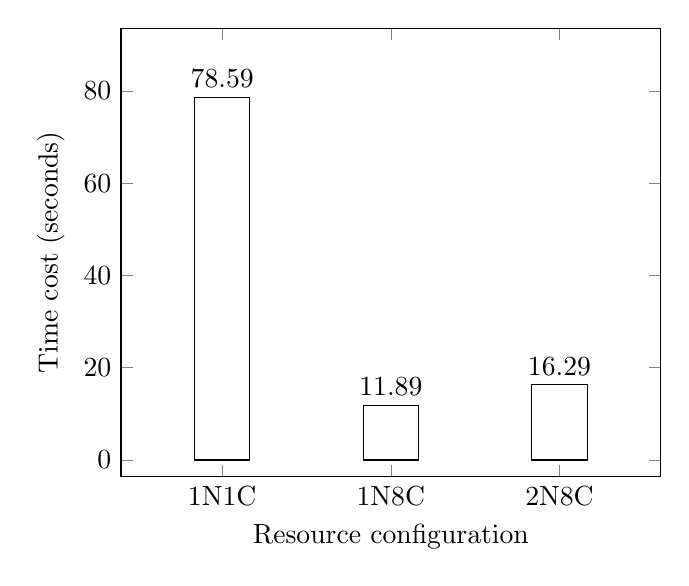
\begin{tikzpicture}
\begin{axis}[
    ylabel={Time cost (seconds)},
    xlabel={Resource configuration},
    ymin=0, ymax=90,
    enlarge x limits=0.3,
    enlarge y limits=0.04,
    bar width=20pt,
    symbolic x coords={1N1C, 1N8C, 2N8C},
    xtick=data,
    nodes near coords
    ]
    
\addplot[ybar] coordinates {(1N1C, 78.59) (1N8C, 11.89) (2N8C, 16.29)};
\end{axis}
\end{tikzpicture}
\end{center}
\caption{Execution time (s) of application on \texttt{bigTwitter.json}; \texttt{1N1C} stands for 1 node 1 core, \texttt{1N8C} stands for 1 node 8 cores and \texttt{2N8C} stands for 2 nodes and 8 cores (with 4 cores per node)}
\label{exe}
\end{figure}

Figure~\ref{exe} presents the time costs. 
It can be seen that 1N1C ran the longest at 78.59 seconds. 
The costs for 1N8C and 2N8C are similar, with the time spent by 1N8C being slightly shorter at 11.89 seconds when compared to 16.29 seconds for 2N8C. 
Both are about 5 times faster than 1N1C.

The cost of 1N1C can be considered to the baseline. % as it ran on a single node with a single core. 
With 8 cores in parallel, say 1N8C, the time cost is reduced. 
However, the theoretical speedup of 8 is not achievable as there are parts of the program which cannot be easily parallelised (e.g. the merging of results). 
Additionally, there are various overheads associated with the OpenMP and MPI runtime libraries and various I/O operations (e.g. network communication for message passing and reading \texttt{bigTwitter.json}). 

Finally, it is unclear why 2N8C is somewhat slower than 1N8C, though it can be seen from the \texttt{/usr/bin/time} output that the CPU utilisation for \texttt{2N8C} was lower. 
Though further experimentation and measurements will be required, it is possible that the program was often blocked by I/O operations. 

\section{Further improvements}
\label{improvements}
% Further improvements are suggested:

\begin{itemize}
    \item
    Currently, the issue of load imbalance between nodes is not addressed. 
    This could be a problem when nodes are heterogeneous, as faster nodes will be idle when waiting for slower nodes to finish. 
    Possible solutions include using a distributed task queue (in place of MPI) or having the master node manage and distribute smaller work units. 
    However, it is important to note that the tradeoff between computation time and communication time (due to network overhead) must be examined when such alternatives are considered. 
    \item
    Optimisations can be applied to the merging of results at the process level to further reduce network communication. 
    % An algorithm can be applied such that less data is sent. 
    \item
    Further investigation can be made on file reading. 
    It is unknown whether it would be better to have multiple threads reading the file concurrently or a single thread which is responsible for reading the file and distributing the data to other threads. 
    
    The current 200MB chunk size is also rather arbitrary and requires further investigation. 
\end{itemize}


\section{Conclusion}
In this report, a parallelized application for processing a large Twitter dataset was introduced. The performance characteristics of the application under different resource configurations was described and analysed. %  was executed on different resource configurations. 

%From the results, we can see that parallel computing on Spartan solves a problem within a shorter time. 
From the results, it can be seen that because the application has been parallelized, it is able to take advantage of the multi-node and multi-core distributed-memory environment that is provided by Spartan. 
However, care must be taken when configuring resources, which includes network and disk I/O,  as well as node and core distributions.
It is worthwhile to read the documentation of a HPC cluster to choose the best group of nodes or partition to run the application under. 
% Also, a developer benefits from the documentation of a HPC cluster to choose the proper group to run the application.

% \begin{itemize}
% \item benefits of cluster and cloud computing
% \item extra cost of them
% \item bottlenecks it has
% \end{itemize}

\begin{thebibliography}{9}
\bibitem{spartan} 
Lev Lafayette, Greg Sauter, Linh Vu, Bernard Meade, "Spartan Performance and Flexibility: An HPC-Cloud Chimera", OpenStack Summit, Barcelona, October 27, 2016. \href{http://doi.org/10.4225/49/58ead90dceaaa}{doi.org/10.4225/49/58ead90dceaaa}

\bibitem{spartan2}
“Spartan Documentation,” Spartan Documentation. [Online]. Available: https://dashboard.hpc.unimelb.edu.au/. [Accessed: 14-Apr-2020].
\end{thebibliography}

\end{document}

